\documentclass[11pt]{article}
\usepackage[margin=1in]{geometry}
\usepackage{graphicx}
\usepackage{booktabs}
\usepackage{amsmath}
\usepackage[hidelinks]{hyperref}

\title{Comparability-aware screening of legacy mercury and lead enrichment
in European soil profiles from harmonized open geochemical data}

\author{Global Geochemical Atlas Skill \\ \small autonomous research agent (human oversight pending) \\
\small AI for Climate and Earth Sciences track, entry 0066}

\date{August 18, 2026 \\ \vspace{4pt} \small Preprint draft (screening-level results; human review pending)}

\begin{document}
\maketitle

\begin{abstract}
High-impact environmental assessments increasingly train on aggregated public
geochemical measurements, yet assembling such data remains a years-long manual
effort, and naive pooling across surveys is unsafe: we show that a single
element (Cr) measured on the same European soil samples differs by a factor of
$\sim$3 between acid-digestion inductively coupled plasma (ICP) and total
X-ray fluorescence (XRF) determinations. Here we
demonstrate an autonomous, fully reproducible pipeline that acquires
29 open sources into a 191{,}715-record standardized geochemical database with
record-level provenance (SHA-256 chained) and four-dimensional confidence
scores, then derives method-stratified, site-paired screening statistics.
Applied to the European FOREGS baseline (Forum of European Geological
Surveys), the pipeline quantifies the
anthropogenic legacy fingerprint in soil profiles: topsoil/subsoil
concentration ratios are elevated for the atmospherically deposited metals Hg
(median 1.36, 95\% bootstrap confidence interval (CI) 1.30--1.44,
$n{=}392$ site pairs, Wilcoxon
$p{=}6{\times}10^{-29}$) and Pb (1.24, 1.19--1.30, $n{=}389$), but not for the
geogenic controls Ni (0.95) and Cr (0.98). Organic (humus) horizons accumulate
Hg 5.3-fold (95\% CI 3.9--5.8; 95\% of sites $>$1.5) and Pb 2.2-fold over
subsoil, while Ni is depleted to 0.29, isolating the vegetation-mediated
atmospheric pathway. An independent-survey replication on U.S. Geological
Survey (USGS) conterminous-US A/C horizon pairs reproduces the geogenic
control behavior (Ni 0.92,
Cu 1.02); horizon-paired Hg and Pb are absent from the ingested US open
sources, a gap the pipeline emits as a machine-actionable sampling priority.
Median paired topsoil Hg (43.9~$\mu$g\,kg$^{-1}$) agrees with the independent
estimate from the EU LUCAS soil survey (38.3~$\mu$g\,kg$^{-1}$). Relative to
the reference
atlas ratios computed in 2006 from outlier-inclusive means, our
method-stratified robust estimates are lower but concordant in direction and
ranking, and add uncertainty quantification, significance testing, and
exclusion accounting. The paired enrichment surface peaks in a belt near
48$^{\circ}$N; because the harmonized FOREGS slice ends near 52$^{\circ}$N, the
northward continuation is untestable from currently ingested open data --- a
concrete, prioritized acquisition target. These outputs directly address the
harmonization, background-separation and coverage limitations that the
Minamata Convention's ongoing effectiveness evaluation reports for global
soil monitoring. All results derive deterministically from a frozen snapshot
and a single analysis script.
\end{abstract}

\section{Introduction}

Continental- and global-scale environmental assessments are increasingly
data-driven: machine-learning models trained on tens of thousands of
aggregated public measurements now underpin global groundwater arsenic risk
mapping \cite{podgorski2020}, and deep-learning maps of European topsoil
mercury are built from $>$21{,}000 harmonized samples of the EU Land
Use/Cover Area frame Survey (LUCAS) \cite{ballabio2021}. The rate-limiting step in such studies is rarely the
model; it is the assembly of comparable, quality-controlled, provenance-complete
observations from heterogeneous open sources --- an effort that typically takes
expert teams months to years, and that is difficult to audit or reproduce after
the fact \cite{reimann2005}.

Mercury is a paradigmatic target for such infrastructure. Soils are the
largest terrestrial Hg reservoir, with climate and vegetation as primary
storage drivers \cite{wang2019}. Atmospheric deposition of gaseous elemental
Hg, mediated by vegetation uptake and litterfall, is the dominant input
pathway \cite{obrist2017,jiskra2018}, and the resulting legacy pool is
climate-sensitive: warming-driven turnover of soil organic matter can
remobilize accumulated Hg to waters and the atmosphere
\cite{obrist2017,schuster2018,schaefer2020}, and observation-driven models
project that warming-induced vegetation greening may raise temperate soil Hg
levels faster than emission controls offset them \cite{liu2024}. Quantifying
how much legacy Hg (and Pb, its co-deposited tracer) is stored in surface
relative to deep soil horizons is therefore both a contamination-screening
and a climate-relevant question --- and a timely one: the Minamata
Convention's ongoing effectiveness evaluation reports that available soil-Hg
data cannot yet be compared across surveys or separated into background and
anthropogenic components \cite{unep2025}, and the EU Soil Monitoring Law (in
force December 2025) now mandates harmonized, comparable soil-contamination
monitoring \cite{eusml2025}. The Geochemical Atlas of Europe, produced by
the Forum of European Geological Surveys (FOREGS) \cite{salminen2005},
provides the canonical paired-horizon baseline and has underpinned
continent-scale geostatistical analyses of soil heavy metals
\cite{lado2008}; its interpretive volume reported
topsoil/subsoil ratios (Hg 1.66, Pb 1.36) computed as arithmetic means of
individual site ratios, outliers included, with analytical methods pooled
\cite{devos2006}.

This paper makes three contributions. \textbf{(i) Infrastructure.} We
demonstrate an autonomous agent pipeline (the \emph{Global Geochemical Atlas}
skill) that acquires, normalizes, spatially registers, quality-controls and
provenance-chains open geochemical data into a standardized database, and then
--- in the same deterministic run --- derives research products: comparability
cohorts, environmental context tables, and prioritized data-gap queues.
\textbf{(ii) Screening science.} Using method-stratified, site-paired robust
statistics on that database, we re-derive the European legacy-metal
fingerprint with uncertainty quantification and cross-continental replication,
quantify organic-horizon Hg accumulation, and verify external consistency
against the independent LUCAS survey. \textbf{(iii) Negative knowledge.} We
show why naive pooling fails (a 3$\times$ same-sample method artifact for Cr)
and emit the resulting comparability constraints and coverage gaps as
machine-actionable outputs rather than prose caveats.

We emphasize scope: all results are screening-level statements about
harmonized open observations. Ratios above unity indicate surface enrichment
consistent with atmospheric legacy inputs; they are not, by themselves,
attributions of pollution sources, health risk, or climate response.

\section{Materials and methods}

Figure~\ref{fig:pipeline} summarizes the workflow: an autonomous acquisition
and harmonization pipeline produces a standardized, confidence-scored
database and derived research products; this study then applies a
site-paired, method-stratified screening design to the paired-horizon subset.

\begin{figure}[t]
\centering
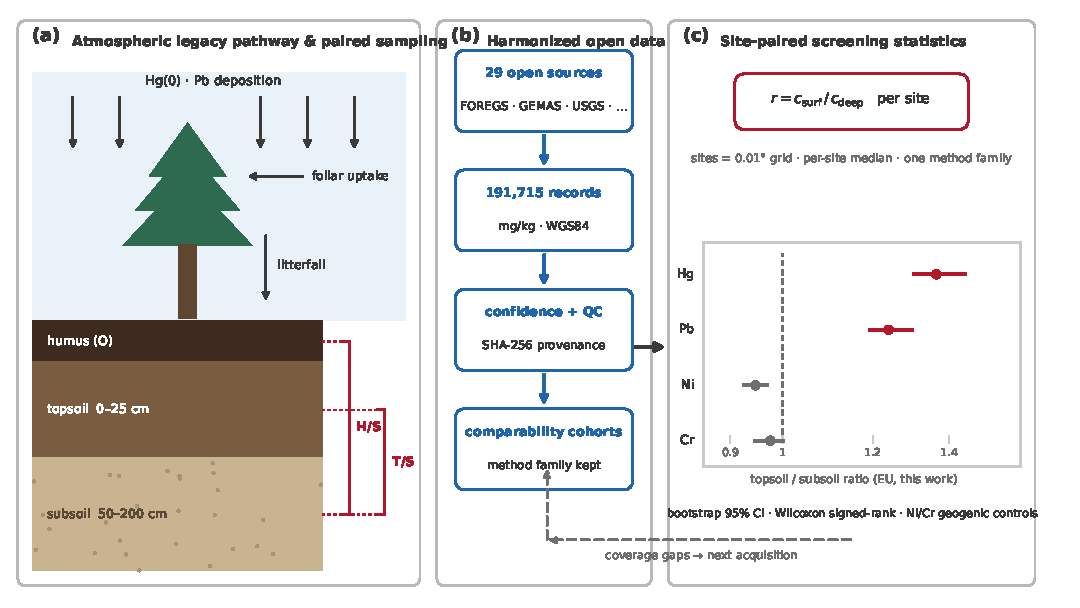
\includegraphics[width=\linewidth]{fig0_pipeline.pdf}
\caption{Methods overview; numbered badges give the reading order.
Top band (left to right): the autonomous pipeline
from open-source acquisition (license audit, SHA-256 provenance) through
unit/coordinate normalization, confidence scoring and quality control (QC)
to deterministic
research products; comparability cohorts feed the screening study. Bottom
band (right to left): the present study's site-paired screening design ---
per-site medians within a single method family on paired horizons
(humus/topsoil/subsoil; H/S and T/S ratios, A/C for the US replication),
bootstrap confidence intervals and Wilcoxon tests with Ni/Cr as geogenic
controls --- and its outputs. The dashed return edge closes the loop:
coverage gaps identified by the study are emitted as machine-actionable
acquisition priorities for the next pipeline run.}
\label{fig:pipeline}
\end{figure}

\subsection{Harmonized database}
A production run of the pipeline (2026-08-15) ingested 29 open sources across
soil, sediment and water into 191{,}715 standardized measurement records
(41{,}508 unique sample identifiers; seven analytes: As, Cr, Cu, Hg, Ni, Pb,
Zn). Each
record carries normalized value and unit (mg\,kg$^{-1}$ for solids), WGS84
coordinates with transform lineage, sample type, method family,
digestion/extraction, license and source locator, file SHA-256, and a
four-dimensional operational confidence object (source evidence, analytical
readiness, spatial usability, workflow usability). The snapshot analyzed here
is frozen (\texttt{geochemistry.csv},
SHA-256 \texttt{e3616e88b6f5\ldots}); the downstream analysis is a single
deterministic script with a seeded bootstrap.

\subsection{Paired-horizon design}
For each element we selected a single method family per survey to avoid
mixing analytical populations: Hg by atomic absorption spectrometry (AAS;
identical in both FOREGS horizons), Pb/As/Cu/Ni by inductively coupled
plasma mass spectrometry (ICP-MS), Cr/Zn by XRF, and inductively coupled
plasma optical emission spectrometry (ICP-OES) for the USGS conterminous-US
soil survey \cite{smith2013}. Records
lacking positive values or canonical coordinates were excluded. Sites were
formed by rounding coordinates to 0.01$^{\circ}$ and taking per-site medians;
surface/deep ratios were computed at sites where both horizons exist
(FOREGS topsoil 0--25 cm vs.\ subsoil C-horizon 50--200 cm; FOREGS humus (O)
vs.\ subsoil; USGS A-horizon vs.\ C-horizon). For each element we report the
median ratio, a 2{,}000-draw bootstrap 95\% confidence interval (CI) of the
median, the fraction of
sites with ratio $>$1.5, and a two-sided Wilcoxon signed-rank test on log
ratios. Sensitivity analyses repeat the procedure at 0.1$^{\circ}$ rounding
and, for Pb, with the alternative ICP-OES determinations. US As (available
only by AAS) was omitted from the US panel for method-family consistency.

\emph{Relation to enrichment-factor practice.} We deliberately use direct
same-site surface/deep ratios rather than crustal- or
reference-element-normalized enrichment factors (EFs). Classical EFs inherit the
well-documented sensitivity to the choice of reference element and crustal
composition \cite{reimann2005}; moreover, conservative reference elements
(Al, Ti, Zr) are not part of the seven-analyte harmonized set. The paired
design cancels first-order lithological variation by construction (both
horizons share parent material at a site), and residual pedogenic
redistribution is bounded empirically by the behavior of the lithogenic
controls Ni and Cr, which remain at or below unity in both surveys.

\subsection{Comparability guard}
Cohort construction in the pipeline stratifies by element, medium, sample
type, grain fraction, measurement basis, method family, digestion and unit
layer. The empirical motivation is measurable within-survey: on the same
FOREGS topsoil samples, median Cr is 27 mg\,kg$^{-1}$ by acid-digestion
ICP-OES versus 74 mg\,kg$^{-1}$ by total XRF ($n{=}446$ each; subsoil 29 vs.\
79); agricultural soils from the GEMAS survey (Geochemical Mapping of
Agricultural and Grazing Land Soils) \cite{reimann2014} show 20.1 (ICP-MS,
aqua regia) versus 62.0
(XRF) mg\,kg$^{-1}$ ($n{=}2{,}224$ each). Any cross-survey comparison that
ignores this stratification inherits a $\sim$3$\times$ artifact exceeding most
signals of interest.

\section{Results}

\subsection{Anthropogenic legacy fingerprint in paired horizons}
Figure~\ref{fig:forest} and Table~\ref{tab:ratios} summarize the paired
ratios. In Europe, the two canonical atmospheric-legacy metals are clearly
elevated in topsoil relative to subsoil: Hg 1.364 (95\% CI 1.303--1.444;
41.3\% of 392 site pairs $>$1.5; $p{=}6.4{\times}10^{-29}$) and Pb 1.239
(1.194--1.299; 28.3\% of 389; $p{=}1.7{\times}10^{-35}$). The mildly
anthropogenic As, Cu and Zn sit at 1.03--1.06 (significant but small), while
the geogenic controls bracket unity: Cr 0.976 (not significant, n.s.) and
Ni 0.947. The
ordering Hg $>$ Pb $>$ (As $\approx$ Cu $\approx$ Zn) $>$ Cr $\approx$ Ni
matches the expected volatility- and deposition-driven hierarchy of legacy
inputs. Results are invariant to coordinate rounding, and the Pb estimate is
method-robust (ICP-OES 1.286 vs.\ ICP-MS 1.239).

In the independent USGS conterminous-US survey, the same design reproduces
the geogenic control behavior (Ni 0.921, CI 0.894--0.945; Cu 1.020, n.s.) with
a slight Zn surface excess (1.041), on $\sim$658 A/C pairs. Horizon-paired Hg
and Pb do not exist in the ingested US open sources --- see \S\ref{sec:gaps}.

\begin{figure}[t]
\centering
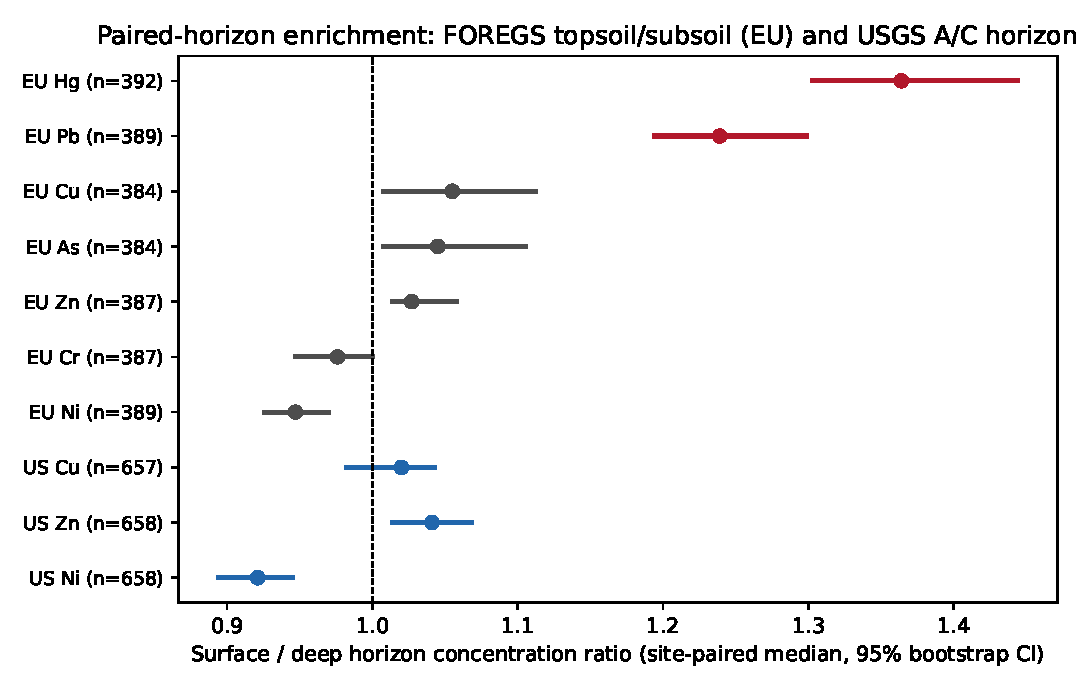
\includegraphics[width=0.92\linewidth]{fig1_forest.pdf}
\caption{Surface/deep concentration ratios at site-paired locations:
FOREGS topsoil/subsoil (EU, red/grey) and USGS A/C horizons (US, blue).
Points are medians of per-site ratios; bars are 95\% bootstrap CIs of the
median. Method-stratified (Hg: AAS; Pb, As, Cu, Ni: ICP-MS; Cr, Zn: XRF;
US panel: ICP-OES). Dashed line: no enrichment.}
\label{fig:forest}
\end{figure}

\begin{table}[t]
\centering\small
\caption{Paired surface/deep concentration ratios: median, 95\% bootstrap CI
of the median, share of site pairs with ratio $>$1.5, and two-sided Wilcoxon
signed-rank $p$. Panels --- EU T/S: FOREGS topsoil/subsoil; EU H/S: FOREGS
humus/subsoil; US A/C: USGS A-horizon/C-horizon.}
\label{tab:ratios}
\begin{tabular}{llrrrrl}
\toprule
Panel & Element & $n$ pairs & Median & 95\% CI & $>$1.5 & $p$ \\
\midrule
EU T/S & Hg & 392 & 1.364 & 1.303--1.444 & 41.3\% & $6.4{\times}10^{-29}$ \\
EU T/S & Pb & 389 & 1.239 & 1.194--1.299 & 28.3\% & $1.7{\times}10^{-35}$ \\
EU T/S & Cu & 384 & 1.055 & 1.008--1.112 & 21.1\% & $4.4{\times}10^{-4}$ \\
EU T/S & As & 384 & 1.045 & 1.008--1.105 & 18.2\% & $5.4{\times}10^{-3}$ \\
EU T/S & Zn & 387 & 1.027 & 1.014--1.058 & 15.0\% & $6.5{\times}10^{-4}$ \\
EU T/S & Cr & 387 & 0.976 & 0.947--1.000 & 9.6\% & 0.064 \\
EU T/S & Ni & 389 & 0.947 & 0.926--0.970 & 9.5\% & $1.2{\times}10^{-3}$ \\
\midrule
EU H/S & Hg & 75 & 5.256 & 3.885--5.811 & 94.7\% & $2.1{\times}10^{-13}$ \\
EU H/S & Pb & 59 & 2.166 & 1.667--2.563 & 67.8\% & $1.1{\times}10^{-7}$ \\
EU H/S & Cu & 59 & 0.649 & 0.583--1.031 & 28.8\% & 0.167 \\
EU H/S & Ni & 59 & 0.292 & 0.233--0.351 & 5.1\% & $8.0{\times}10^{-10}$ \\
\midrule
US A/C & Zn & 658 & 1.041 & 1.014--1.068 & 19.9\% & $3.2{\times}10^{-5}$ \\
US A/C & Cu & 657 & 1.020 & 0.982--1.043 & 17.4\% & 0.277 \\
US A/C & Ni & 658 & 0.921 & 0.894--0.945 & 6.1\% & $6.9{\times}10^{-18}$ \\
\bottomrule
\end{tabular}
\end{table}

\subsection{Organic horizons isolate the atmospheric pathway}
Humus (O-horizon) samples sharpen the contrast (Fig.~\ref{fig:horizons};
Table~\ref{tab:ratios}). Relative to subsoil at the same sites, humus is
enriched 5.26-fold in Hg (95\% CI 3.89--5.81; 94.7\% of 75 pairs $>$1.5) and
2.17-fold in Pb, while lithogenic Ni is \emph{depleted} to 0.29 --- an
18-fold behavioral separation between Hg and Ni across one soil profile.
Absolute levels fall in the expected order (site-median Hg: humus 0.204,
topsoil 0.044, subsoil 0.031 mg\,kg$^{-1}$). This is the vegetation-pump
signature --- foliar uptake of atmospheric Hg(0) delivered to soil by
litterfall \cite{jiskra2018,obrist2017} --- made visible directly in
harmonized open survey data, without isotopes or flux towers.

\begin{figure}[t]
\centering
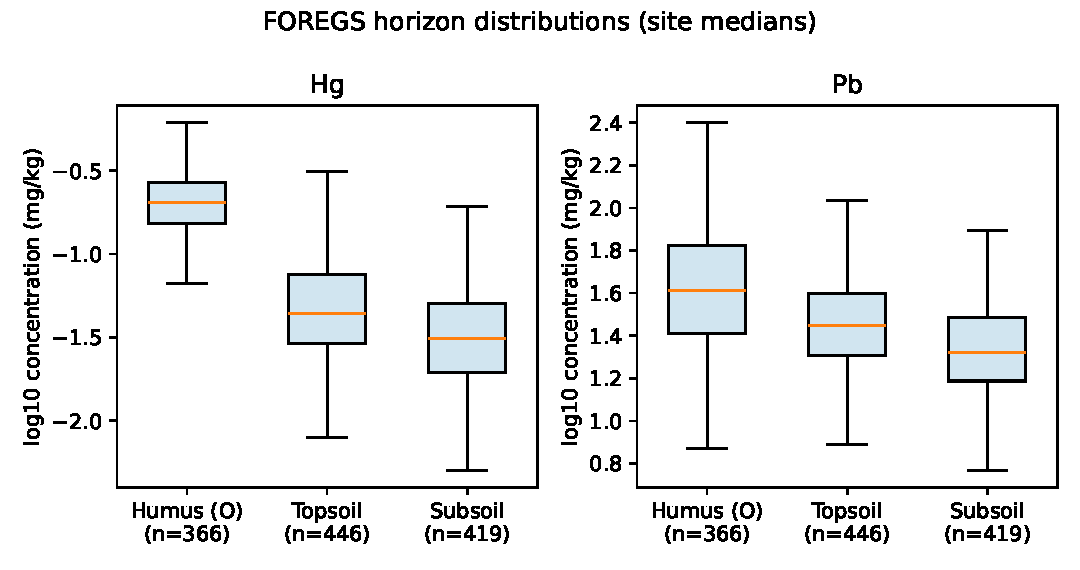
\includegraphics[width=0.9\linewidth]{fig3_horizons.pdf}
\caption{Site-median concentration distributions by FOREGS horizon
(log10 mg\,kg$^{-1}$; boxes: interquartile range, IQR; whiskers: 1.5 IQR;
outliers hidden).
Hg and Pb increase monotonically toward the surface organic horizon.}
\label{fig:horizons}
\end{figure}

\subsection{Spatial structure and the 48$^{\circ}$N belt}
Mapping per-site log2 Hg ratios (Fig.~\ref{fig:map}) reveals coherent
structure rather than noise: the strongest 2$^{\circ}$ aggregates (5--9 pairs
each, median log2 ratio 0.73--1.49, i.e.\ up to $\sim$2.8$\times$) form a belt
near 48$^{\circ}$N spanning eastern France, southern Germany, Austria and
Slovakia, with a secondary cluster in central Italy. The belt is consistent
with combined industrial-era deposition and forest-mediated uptake, and with
the independent LUCAS-based observation that European topsoil Hg increases
with latitude and vegetation activity \cite{ballabio2021}. We flag it as a
screening pattern: attribution requires deposition modeling and land-cover
covariates, which the pipeline exposes as declared (not yet ingested)
interfaces.

\begin{figure}[t]
\centering
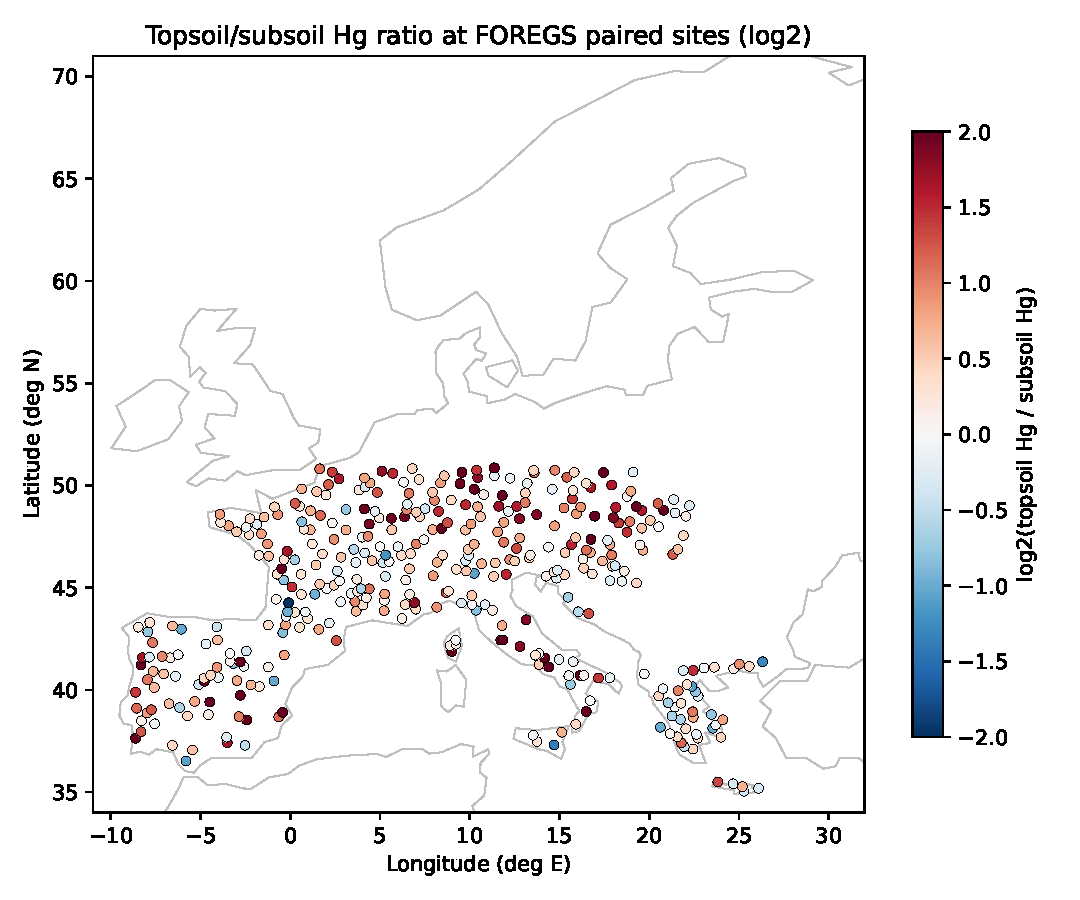
\includegraphics[width=0.78\linewidth]{fig2_hg_map.pdf}
\caption{Topsoil/subsoil Hg ratio (log2) at FOREGS paired sites. Red:
surface enrichment. The harmonized FOREGS slice contains no paired sites
north of 52$^{\circ}$N (see \S\ref{sec:gaps}). Land outline: Natural Earth.}
\label{fig:map}
\end{figure}

\subsection{Agreement with, and sharpening of, the reference atlas}
The 2006 atlas interpretation reported topsoil/subsoil ratios of 1.660 (Hg)
and 1.364 (Pb) as arithmetic means of site ratios, outliers included, methods
pooled \cite{devos2006}. Our method-stratified medians are lower (1.364 and
1.239) --- as expected when heavy right tails are not allowed to dominate ---
but concordant in direction and in the ranking of elements. The added value
of the automated re-derivation is (i) uncertainty quantification and
significance testing, (ii) explicit method stratification (motivated by the
3$\times$ Cr artifact), (iii) full exclusion accounting from raw records to
final pairs, and (iv) single-command reproducibility. External consistency:
our paired-site topsoil Hg median (43.9~$\mu$g\,kg$^{-1}$) is within 15\% of
the independent LUCAS deep-learning estimate for EU topsoil
(38.3~$\mu$g\,kg$^{-1}$) \cite{ballabio2021}.

\subsection{Coverage gaps as first-class outputs}
\label{sec:gaps}
Three gaps discovered by this analysis are emitted by the pipeline as
machine-actionable priorities rather than prose limitations:
(1) \emph{Nordic truncation}: the ingested FOREGS soil slice ends at
50.9$^{\circ}$N (topsoil) / 52.5$^{\circ}$N (subsoil), so the northward
continuation of the 48$^{\circ}$N belt --- where the vegetation-pump
hypothesis predicts continued increase \cite{ballabio2021} --- is currently
untestable from the harmonized data; Fennoscandian acquisition is queued in
the run's coverage-repair tasks.
(2) \emph{US legacy metals}: no horizon-paired Hg or Pb exists in the ingested
US open sources, precluding cross-continental replication of the headline
result; the sampling-priority layer records this as a candidate acquisition
or field target.
(3) \emph{Cross-source comparability}: at strict cohort granularity the run
yields zero multi-source comparable cohorts (290 sample-sufficient cohorts are
all single-source dominated), so every cross-survey statement in this paper is
framed as replication across surveys, never pooling.

\section{Discussion}

\textbf{What the numbers support.} Harmonized open data suffice to quantify,
with uncertainty, a continental legacy-metal fingerprint: European surface
soils carry a measurable stock of atmospherically delivered Hg and Pb
relative to their own subsoil, concentrated where organic matter accumulates.
The humus Hg enrichment (5.3$\times$) dwarfs the mineral topsoil signal
(1.36$\times$), consistent with organic-matter binding as the storage
mechanism \cite{obrist2017,jiskra2018}.

\textbf{Position within the current frontier.} Three active research and
policy programs need exactly the quantities produced here. (i)~The Minamata
Convention's first effectiveness evaluation: its Open-Ended Scientific Group
reports that available soil-Hg data are sparse, cover incompatible periods,
cannot be compared across surveys for lack of consistent
sampling/extraction/analysis, and do not separate background from
anthropogenic levels --- and the European dataset it relies on is the same
FOREGS survey harmonized here \cite{unep2025}. Our comparability cohorts,
method-stratified paired ratios (a direct background/anthropogenic
separation) and machine-readable coverage gaps address each stated
limitation. (ii)~The EU Soil Monitoring Law, in force since December 2025,
mandates a harmonized soil-health monitoring framework including
contamination \cite{eusml2025}; a confidence-scored, provenance-chained
baseline of the kind assembled here is the natural substrate for its
cross-border comparability requirement. (iii)~The soil--climate Hg
frontier: soils store the largest terrestrial Hg reservoir, with climate and
vegetation as primary storage drivers \cite{wang2019}; recent
observation-driven modeling indicates warming-induced vegetation greening
may aggravate soil Hg levels faster than emission controls can offset
\cite{liu2024}, and permafrost projections put remobilization on the agenda
of land-surface models now being extended with explicit Hg cycles
\cite{schaefer2020}. Those models are evaluated against regional surface-Hg
maps and vertical profiles --- precisely the site-paired, method-controlled
ratio tables published here, for the temperate mid-latitudes where
\cite{liu2024} project the largest increases.

\textbf{New questions generated.} (Q1) \emph{Climate remobilization}: given
organic-horizon Hg stocks 5$\times$ subsoil levels, what fraction is
re-emitted or exported under warming-driven soil-carbon turnover in temperate
Europe --- the mid-latitude counterpart to the permafrost Hg question
\cite{schuster2018,schaefer2020} and the observational face of the
greening--Hg feedback \cite{liu2024}? The paired-site table published here
is a ready-made constraint set for such models. (Q2) \emph{Belt attribution}: does
the 48$^{\circ}$N enrichment belt follow historical deposition fields,
forest cover, or soil organic carbon --- and does it continue into
Fennoscandia? (Q3) \emph{Comparability standards}: with a 3$\times$
same-sample method artifact and zero multi-source cohorts, what minimum
metadata and inter-method transfer models would make global soil-metal data
poolable? Each question maps onto a concrete pipeline extension (declared
covariate interfaces; Nordic acquisition; cohort-transfer calibration).

\textbf{Limitations.} FOREGS density is one site per $\sim$4{,}700 km$^2$;
ratios conflate pedogenic redistribution with anthropogenic input (mitigated,
not eliminated, by the Ni/Cr controls and the humus contrast); no dating or
isotopes constrain input chronology; humus pairing recovers only 75 Hg sites;
and all statements inherit the licenses and quality of the upstream surveys.
These results are screening products intended to seed, not replace,
process studies.

\textbf{Reproducibility as a scientific control.} Every number above is
regenerated by one script on one frozen snapshot with a seeded bootstrap;
two independent executions produce byte-identical outputs. We regard this
property --- rare in data-assembly-heavy environmental work --- as the main
methodological claim of the paper, and the screening results as its
demonstration.

\section{Conclusion}
An autonomous pipeline can turn scattered open geochemical sources into
research-grade, comparability-aware evidence and derive from it a defensible
continental screening result, its uncertainty, its external consistency
checks, and --- critically --- the exact boundaries of what the data cannot yet
support, expressed as prioritized acquisition targets. We propose this
data-to-question loop as a template for AI-assisted earth-science
infrastructure.

\section*{Data and code availability}
Input sources (with licenses recorded per record in the database):
FOREGS Geochemical Atlas of Europe topsoil/subsoil/humus data
(Geological Survey of Finland; research use with attribution)
\cite{salminen2005,devos2006};
USGS conterminous US soil geochemistry, Data Series 801 (public domain,
doi:10.3133/ds801) \cite{smith2013};
GEMAS agricultural soils (CC-BY-4.0) \cite{reimann2014}.
The frozen standardized snapshot, the analysis script
(\texttt{paper\_analysis.py}), per-site pair tables, result JSON and figure
sources are archived with SHA-256 receipts in the pipeline's
\texttt{research-products/paper-demo-20260817} directory.

\section*{Agent disclosure}
This draft, including data acquisition, harmonization, analysis design,
statistics, figures and text, was produced end-to-end by an AI research agent
operating the Global Geochemical Atlas skill; the human team has not yet
completed review. Screening-level framing is intentional and load-bearing.

\begin{thebibliography}{12}
\bibitem{ballabio2021}
Ballabio, C., Jiskra, M., Osterwalder, S., Borrelli, P., Montanarella, L.,
Panagos, P. (2021). A spatial assessment of mercury content in the European
Union topsoil. \emph{Science of the Total Environment}, 769, 144755.
doi:10.1016/j.scitotenv.2020.144755.

\bibitem{devos2006}
De Vos, W., Tarvainen, T. (chief eds.), et al. (2006). \emph{Geochemical
Atlas of Europe. Part 2: Interpretation of Geochemical Maps, Additional
Tables, Figures, Maps, and Related Publications}. Geological Survey of
Finland, Espoo.

\bibitem{jiskra2018}
Jiskra, M., Sonke, J.E., Obrist, D., et al. (2018). A vegetation control on
seasonal variations in global atmospheric mercury concentrations.
\emph{Nature Geoscience}, 11, 244--250. doi:10.1038/s41561-018-0078-8.

\bibitem{lado2008}
Rodriguez Lado, L., Hengl, T., Reuter, H.I. (2008). Heavy metals in European
soils: a geostatistical analysis of the FOREGS geochemical database.
\emph{Geoderma}, 148, 189--199.

\bibitem{obrist2017}
Obrist, D., Agnan, Y., Jiskra, M., et al. (2017). Tundra uptake of
atmospheric elemental mercury drives Arctic mercury pollution.
\emph{Nature}, 547, 201--204. doi:10.1038/nature22997.

\bibitem{podgorski2020}
Podgorski, J., Berg, M. (2020). Global threat of arsenic in groundwater.
\emph{Science}, 368, 845--850. doi:10.1126/science.aba1510.

\bibitem{reimann2005}
Reimann, C., de Caritat, P. (2005). Distinguishing between natural and
anthropogenic sources for elements in the environment: regional geochemical
surveys versus enrichment factors. \emph{Science of the Total Environment},
337, 91--107.

\bibitem{reimann2014}
Reimann, C., Birke, M., Demetriades, A., Filzmoser, P., O'Connor, P. (eds.)
(2014). \emph{Chemistry of Europe's Agricultural Soils} (GEMAS).
Geologisches Jahrbuch B102/B103, Schweizerbart, Stuttgart.

\bibitem{salminen2005}
Salminen, R. (chief ed.), et al. (2005). \emph{Geochemical Atlas of Europe.
Part 1: Background Information, Methodology and Maps}. Geological Survey of
Finland, Espoo.

\bibitem{schuster2018}
Schuster, P.F., Schaefer, K.M., Aiken, G.R., et al. (2018). Permafrost stores
a globally significant amount of mercury. \emph{Geophysical Research
Letters}, 45, 1463--1471.

\bibitem{schaefer2020}
Schaefer, K., Elshorbany, Y., Jafarov, E., Schuster, P.F., Striegl, R.G.,
Wickland, K.P., Sunderland, E.M. (2020). Potential impacts of mercury
released from thawing permafrost. \emph{Nature Communications}, 11, 4650.
doi:10.1038/s41467-020-18398-5.

\bibitem{smith2013}
Smith, D.B., Cannon, W.F., Woodruff, L.G., Solano, F., Kilburn, J.E., Fey,
D.L. (2013). \emph{Geochemical and mineralogical data for soils of the
conterminous United States}. U.S. Geological Survey Data Series 801.
doi:10.3133/ds801.

\bibitem{wang2019}
Wang, X., Yuan, W., Lin, C.-J., Zhang, L., Zhang, H., Feng, X. (2019).
Climate and vegetation as primary drivers for global mercury storage in
surface soil. \emph{Environmental Science \& Technology}, 53(18),
10665--10675. doi:10.1021/acs.est.9b02386.

\bibitem{liu2024}
Guo, W., Liu, M., Zhang, Q., Deng, Y., Chu, Z., Qin, H., Li, Y., Liu, Y.-R.,
Zhang, H., Zhang, W., Tao, S., Wang, X. (2024). Warming-induced vegetation
greening may aggravate soil mercury levels worldwide. \emph{Environmental
Science \& Technology}, 58(34), 15078--15089. doi:10.1021/acs.est.4c01923.

\bibitem{unep2025}
UNEP Minamata Convention on Mercury, Open-Ended Scientific Group (2025).
\emph{Overview of monitoring, emission and release data}
(UNEP/MC/OESG.2/2/Rev.1) and OESG scientific report executive summary.
\url{https://minamataconvention.org}.

\bibitem{eusml2025}
European Commission (2025). \emph{Soil Monitoring Law} (Directive on Soil
Monitoring and Resilience, in force 16 December 2025).
\url{https://environment.ec.europa.eu/topics/soil-health/soil-monitoring-law_en}.
\end{thebibliography}

\end{document}
